\documentclass[11pt]{article}
\usepackage{graphicx}
\begin{document}
\begin{titlepage}
\title{\Huge ECS 171 Final Report}
\author{\huge Aaun Abbas\\\huge Hilal Alsibai\\\huge Christopher Chen\\\huge Miguel Covarrubias\\\huge Jesse Dyer\\\huge Pei Guo\\\huge Alex Kot\\\huge Raymond Lau\\\huge Kent Wang\\\huge Ian Woods}
\maketitle
\end{titlepage}

\section{Abstract}
\paragraph{}
In this project, we compared the effectiveness of several machine learning classifiers at determining forest cover types from cartographic variables. The classifiers we used were artificial neural networks, k nearest neighbors, and random forests. Our results showed that random forests more accurately predicted the correct forest cover type than any other classifier. 
\section{Introduction}
\paragraph{}
Determining forest cover type from purely cartographic variables is important in situations where it is unfeasible or impossible to obtain cover type data through empirical methods. Thus, being able to accurately estimate the cover type of an area is of great interest to forest scientists \cite{blackard00}.  At the same time, the dataset provides a large amount of well structured data (581012 samples with 54 attributes) upon which different machine learning techniques can be tested and compared, making it an attractive dataset for computer scientists \cite{gama03,oza01,giannella,furnkranz,obradovic,klami}.
\section{Methods}
\paragraph{}
We use three different classifiers to determine forest cover type: artificial neural networks, k nearest neighbors, and random forests.
\subsection{Artificial Neural Networks}
\subsection{k Nearest Neighbors}
\subsection{Random Forests}
\paragraph{}
We used Liaw and Wiener's R port \cite{liaw02} of Breiman's random forest algorithm \cite{breiman01}. Before training the classifier on the samples, we preprocessed the data so that the 4 boolean categorical variables that were related to wilderness area were rolled up into a single variable. We did the same for the 40 variables (also boolean categorical) that were related to soil type. This was done in order to speed up the training of the classifier.
\par
The random forest algorithm takes several parameters which control its speed and performance. We used empirical analysis to determine optimal values for these parameters. The first of these was $mtry$, which controls the number of variables that are sampled at each split when building the decision trees. 7 was determined to be the optimal value, as increasing the value past 7 caused almost no change in error, but consumed far more system resources. The other parameter was $ntree$ which controls the number of trees to be generated in the forest. For the same reasons as $mtry$, 40 was found to be the optimal value.
\par
To determine error, we used the OOB (out of bag) error \cite{breiman96}. We used this estimate because it is automatically generated by the algorithm while it runs, and because cross validation is not required when using OOB error, due to the way it is computed \cite{breiman01, breiman96}, which saved us computation time. It has also been shown to be close to an optimal estimate of the generalization error\cite{breiman96}.

\section{Results}
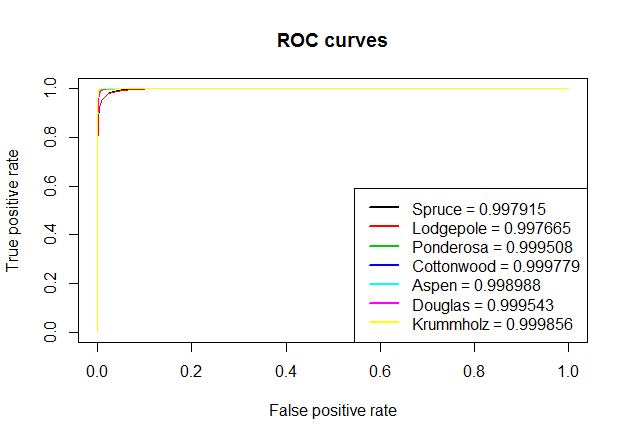
\includegraphics[width=\linewidth]{images/RFROC.png}
This should be an ROC curve.

\section{Discussion}
Why is one classifier better than another?

\section{Conclusion}
In this project we used 3 different classifiers to predict forest cover type based on cartographic variables: artificial neural networks, k nearest neighbors, and random forests. We determined that random forests outperformed the other 2 classifiers. In the future, we may try to examine the performance of these classifiers on other datasets and then compare those results to those given here, or we may use different classifiers on the cover type dataset to see if we can improve our classification accuracy.

\section{Contributions}
Aaun Abbas and Raymond Lau wrote all of the code that was related to random forests. Christopher Chen wrote all parts of the report that were related to random forests.

\pagebreak
\begin{thebibliography}{}
\bibitem{blackard00}
Blackard, Jock A. and Denis J. Dean. 2000. "Comparative Accuracies of Artificial Neural Networks and Discriminant Analysis in Predicting Forest Cover Types from Cartographic Variables." Computers and Electronics in Agriculture 24(3):131-151.

\bibitem{gama03}
Joao Gama and Ricardo Rocha and Pedro Medas. Accurate decision trees for mining high-speed data streams. KDD. 2003.

\bibitem{oza01}
Nikunj C. Oza and Stuart J. Russell. Experimental comparisons of online and batch versions of bagging and boosting. KDD. 2001.

\bibitem{giannella}
Chris Giannella and Bassem Sayrafi. An Information Theoretic Histogram for Single Dimensional Selectivity Estimation. Department of Computer Science, Indiana University Bloomington.

\bibitem{furnkranz}
Johannes Furnkranz. Round Robin Rule Learning. Austrian Research Institute for Artificial Intelligence.

\bibitem{obradovic}
Zoran Obradovic and Slobodan Vucetic. Challenges in Scientific Data Mining: Heterogeneous, Biased, and Large Samples. Center for Information Science and Technology Temple University.

\bibitem{klami}
Arto Klami and Samuel Kaski and Ty n ohjaaja and Janne Sinkkonen. HELSINKI UNIVERSITY OF TECHNOLOGY Department of Engineering Physics and Mathematics Arto Klami Regularized Discriminative Clustering. Regularized Discriminative Clustering.

\bibitem{liaw02}
A. Liaw and M. Wiener (2002). Classification and Regression by randomForest. R News 2(3), 18--22.

\bibitem{breiman01}
Leo Breiman. Random forests. Machine learning 45 (1), 5-32. 2001.

\bibitem{breiman96}
Breiman, Leo. Out-of-bag estimation. Technical report, Statistics Department, University of California Berkeley, Berkeley CA 94708, 1996b. 33, 34, 1996.

\end{thebibliography}
\end{document}